\documentclass[dvipdfmx]{jarticle}
\usepackage{amssymb,amsmath}
\usepackage{tikz}
\usetikzlibrary{calc,shapes}
\usepackage{fancyvrb}
\usepackage{tabularx}
\usepackage{multirow}
\usepackage{wrapfig}
\usepackage{here}
\newcounter{coffee}
\newcounter{bean}
\newcounter{soy}
\hoffset=-25mm \voffset=-25mm
\setlength{\textwidth}{16cm}
\setlength{\textheight}{24cm}
\newcommand{\tteq}{\texttt{=}}
\newcommand{\ttast}{\texttt{*}}
\newcommand{\tti}{\texttt{i}}
\begin{document}
\begin{flushright}
    \verb|2026/12/1|
\end{flushright}
\begin{center}
    {\bf\Large
        2026年度　コンパイラ　定期試験問題
    }
\end{center}

\begin{trivlist}
    \item[$\bullet$] 試験日時：2026/12/1 14:45--16:15\quad {\bf 裏面にも問題があります．}
    \item[$\bullet$] 大問は３題ある．答案用紙に番号を記載して１問ごとに１枚ずつ答案用紙を使うこと．
    \item[$\bullet$] 解答と下書きを明確に区別して書き，
    裏に解答が続くときは，「裏に続く」と書くこと．
    \item[$\bullet$] 下書きと答えがはっきりわかるように記載すること．
\end{trivlist}

\begin{list}{{\bf\large [\arabic{coffee}]}}{\usecounter{coffee}}
    \item 文脈自由文法$G=(\{S,A,B,C\},\{a,b,c\},P,S)$について答えよ．ここで，生成規則集合$P$は以下のものとする．($n:$は規則につけられた番号とする．)
          \[P=\left\{\begin{array}{llll}
                  1: & S\rightarrow AB  & 4: & A\rightarrow \varepsilon \\
                  2: & S\rightarrow bAC & 5: & B\rightarrow a           \\
                  3: & A\rightarrow cA  & 6: & C\rightarrow b           \\
              \end{array}\right\}\]
          \begin{list}{(\arabic{coffee})}{\usecounter{bean}}
              \item $\mathsf{First}_1(A)$ および $\mathsf{Follow}_1(A)$ を求めよ．
              \item $G$の下向き構文解析表を作成せよ．
              \item $G$はLL(1)解析可能かどうか，理由をつけて答えよ．
              \item 図1に示す$G$のLR(0)オートマトンの状態として適当なLR(0)項をうめよ．\\
                    \begin{center}
                        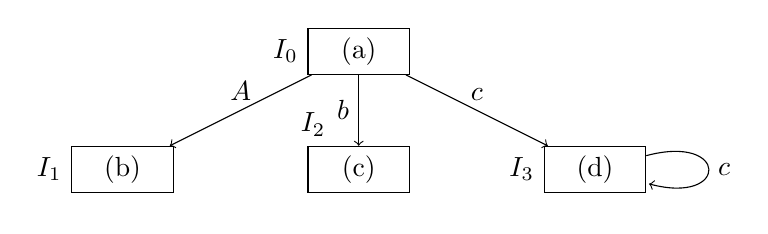
\begin{tikzpicture}
                            \node[draw,label={180:{$I_0$}}] (I0) at (0,0) {\hbox to 3em{\hfill (a)\hfill}};
                            \node[draw,label={180:{$I_1$}}] (I1) at (-3,-1.5) {\hbox to 3em{\hfill (b)\hfill}};
                            \node[draw,label={135:{$I_2$}}] (I2) at (0,-1.5) {\hbox to 3em{\hfill (c)\hfill}};
                            \node[draw,label={180:{$I_3$}}] (I3) at (3,-1.5) {\hbox to 3em{\hfill (d)\hfill}};
                            \path[->] (I0) edge [above] node {$A$} (I1);
                            \path[->] (I0) edge [left] node {$b$} (I2);
                            \path[->] (I0) edge [above] node {$c$} (I3);
                            \path[->] (I3) [loop right] edge [right] node {$c$} (I3);
                        \end{tikzpicture}
                    \end{center}
              \item SLR(1)構文解析表を作成せよ．
              \item $G$はSLR(1)解析可能かどうか，理由をつけて答えよ．
          \end{list}
\end{list}
\end{document}